%
% T�TULO DEL CAP�TULO
%
\chapter{GCVL: GPU Computer Vision Library
	\label{chapter_3}
}

\textbf{GCVL} is a set of software tools and libraries that allow the user to run and implement common Computer Vision algorithms on modern GPUs. It comprises a set of OpenCL and CUDA tools, a Block Matching example algorithm implementation and base classes to implement custom algorithms.

\section{Development Methodology}

Agile software development \cite{agiledev} is a combination of development methods that use iterative and incremental development, where requirements and solutions mature through collaboration between self-organizing, cross-functional teams. The motto of this method is ``embrace change''; that is why it encourages adaptive planning, evolutionary development and delivery, a time-boxed iterative approach, and promotes quick and flexible response to change.

\subsection{Agile manifesto}

In February of 2001, several developers met at Snowbird, Utah resort, to debate different lightweight development methods. They published the \emph{Manifesto for Agile Software Development} \cite{agilemani} to define the approach that is now called agile software development. 

The conclusions that we can reach from the manifesto's items are described below:

\begin{itemize}
\item \textbf{Individuals and Interactions}: In agile development self-organization and motivation are really important. Other values promoted by the manifesto are co-location\footnote{The act of placing multiple individuals within a single location.} and pair programming\footnote{Two programmers work together at one workstation.}.
\item \textbf{Working software}: Working software will be utilized for more purposes than presenting documents to the client.
\item \textbf{Customer collaboration}: The software requirements cannot be fully realized from the beginning of the software development cycle, so being in touch with the customer is really important.
\item \textbf{Responding to change}: Agile development is keen on fast responses to change and continuous development.  
\end{itemize}

More principles are mentioned in the manifesto, some of them are:

\begin{itemize}
\item Customer satisfaction by rapid delivery of useful software.
\item Welcome changes even late in the development.
\item Working software is the principal measure of progress.
\item Maintaining a constant pace.
\item Cooperation between business people and developers. 
\item Build projects around motivated individuals.
\item Attention to technical excellence.
\item Simplicity.
\end{itemize}

Agile methods break down tasks into small increments with minimal planning and normally long-term planning is not directly involved. \emph{Iterations} are short timeframes that typically last from one to four weeks. A team works in each iteration through a full software development cycle; including planning, requirements analysis, design, coding, etc. This minimizes risk and facilitates adaptation to change. An iteration may not add enough new functionalities to warrant a market release, but the objective is to have an available release at the end of each iteration. 

Team composition does not depend on corporate hierarchies or corporate roles of team members. They normally have the responsability of completing tasks that deliver the required functionalities that an iteration requires. How to meet an iteration's objectives is decided individually.

The ``weight'' of the method depends on the type of project, the planning and order of tasks in a generalist project should not be the same as in a research project.  

Agile methods encourage face-to-face communication instead of written documents if possible. Most teams work in an open office (the \emph{bullpen}), which makes this type of communication easier. 

Each agile team contains a customer representative, that ensures that customer needs and company goals are aligned. 

Most agile methods encourage a routine that includes daily face-to-face communication among team members. In a brief session team members tell each other what they achieved the previous day, what they are going to do today and the problems that have appeared. 

As agile development emphasizes on working software as the primary measure of progress and has a clear preference in face-to-face communication this results in less written documentation than other methods. This does not mean that documentation should be disregarded, but that less emphasis is made on documentation because is not needed as much.

\section{Design}

GCVL is developed following an object oriented approach and using the \CC programming language. For GPGPU programming we have chosen OpenCL and CUDA, because of their inter-operation capabilities with OpenGL. This will allow us to process directly data that already resides in the GPU, without having to do expensive memory transfers. Because of the open nature of OpenCL, the software will be able to run on any graphics card vendor (AMD, NVIDIA or Intel) and the SO that the user prefers (Windows, OSX or Unix). For NVIDIA GPUs we have also developed a CUDA implementation, this way users will be able to squish the maximum amount of performance out of the green team's devices. Design patterns have been used as much as possible. This section briefly depicts the high-level design of GCVL in the form of class diagrams.

\subsection{Class diagram}

The high-level design of the \textbf{GCVL} library is depicted in the class diagram of \autoref{class_diag}. In this design, the \textbf{General Tools} module contains utility classes that contain commonly used functions and configuration parameters. In addition, the \textbf{CPU} module contains tools to implement multi-core CPU algorithms using GCVL, examples, template classes, etc.

\begin{figure}[h]
	\centering
	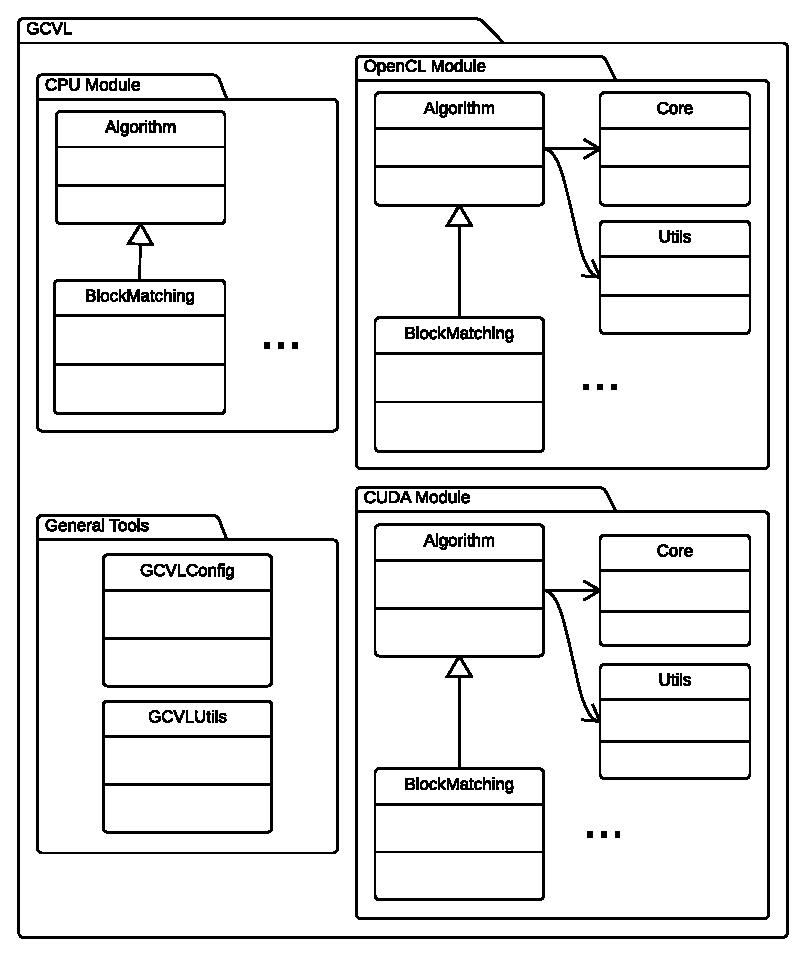
\includegraphics[scale=0.73]{figures/GCVL.pdf}
	\caption{GCVL class diagram.} \label{class_diag}
\end{figure}

Furthermore, the \textbf{OpenCL} module contains classes related to the development of OpenCL algorithms (tools, example algorithms, kernels, etc.).

Finally, the \textbf{CUDA} module resembles the aforementioned module, containing tools, algorithm examples, kernels, etc. It possesses all the classes that are needed to implement CUDA programs in a simple manner.

All of the GPU modules present in GCVL can be compiled on demand using CMake options, so if the CUDA framework or the OpenCL libraries are not needed, they can be deactivated and the rest of the library can be used without any kind of issue.

\subsection{General Tools}

\begin{figure}[h]
	\centering
	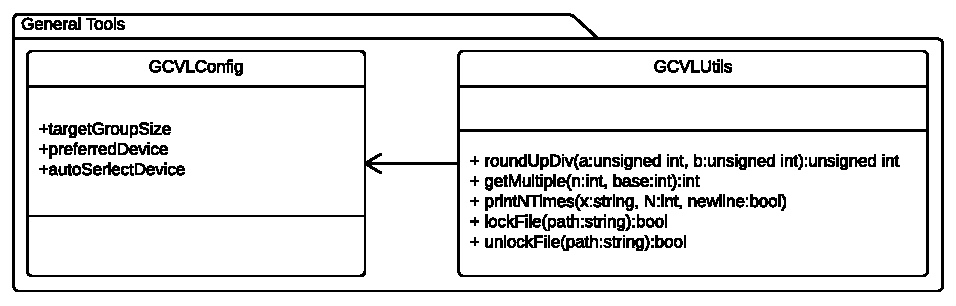
\includegraphics[scale=0.73]{figures/general_tools.pdf}
	\caption{General Tools module class diagram.} \label{general_tools}
\end{figure} 

In the diagram of \autoref{general_tools}, the following classes are the most relevant:

\begin{itemize}
	\item \textbf{GCVLConfig:} This class contains the configuration parameters present in GCVL. For example, the suppression of warnings, constant definitions, etc. 
	\item \textbf{GCVLTools:} Class that contains utility functions used in all the modules present in GCVL, be it CPU or GPU modules. 
\end{itemize}

\subsection{CPU Module}

This is a GPGPU oriented computation library, but it also provides code for multi-core CPUs. The
relevant classes are shown in the class diagram \autoref{cpu_module}:

\begin{itemize}
	\item \textbf{Algorithm:} This base class contains the template for the implementation  of multi-core CPU algorithms in GCVL.
	\item \textbf{BlockMatching:} This class serves as an example of the implementation of a multi-core CPU algorithm in GCVL. 
\end{itemize}

\begin{figure}[h]
	\centering
	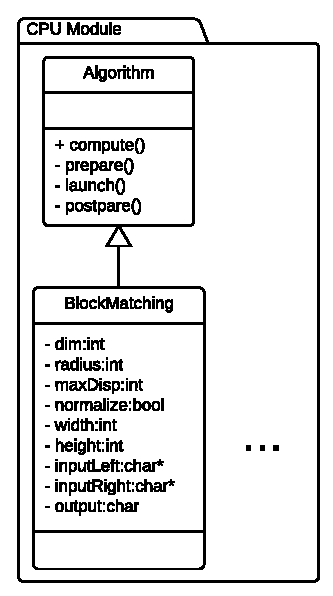
\includegraphics[scale=0.73]{figures/cpu_module.pdf}
	\caption{CPU module class diagram.} \label{cpu_module}
\end{figure} 

\subsection{OpenCL Module}

\begin{figure}[h]
	\centering
	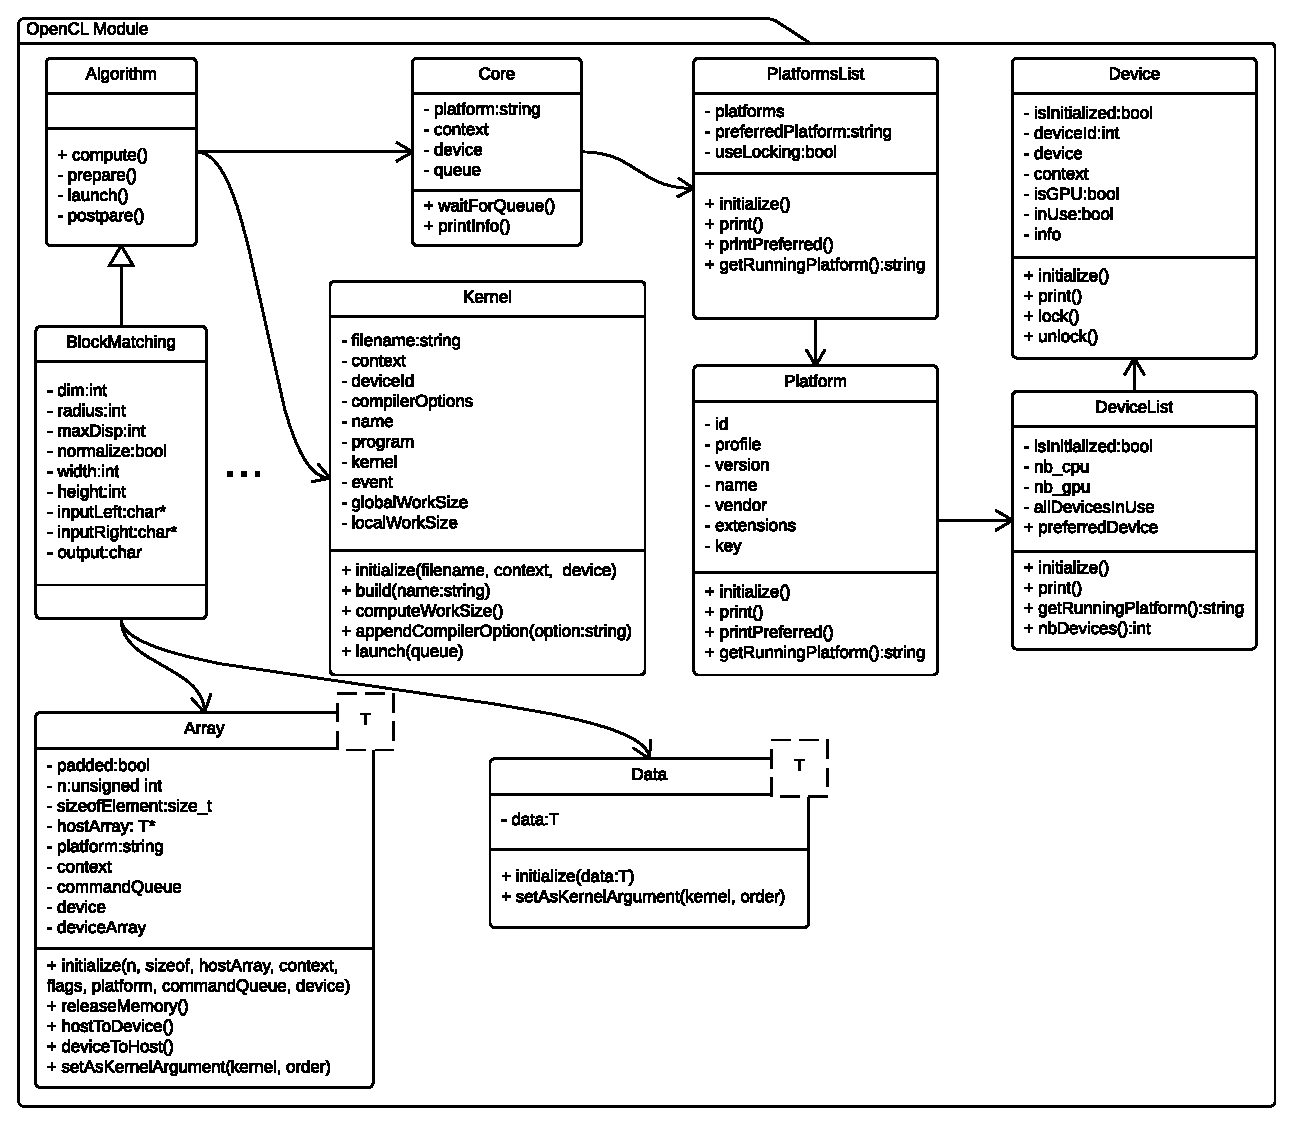
\includegraphics[scale=0.73]{figures/opencl_module.pdf}
	\caption{OpenCL module class diagram.} \label{opencl_module}
\end{figure} 

Since this is a GPU computing library, the first related module is the OpenCL module. In it, classes, algorithms, kernels that belong to the OpenCL implementation are packed together for convenience in the \textbf{opencl} name space. The most significant classes related to the management of the OpenCL algorithms are shown in the class diagram of \autoref{opencl_module}:

\begin{itemize}
	\item \textbf{Algorithm:} This base class contains the template for the implementation  of OpenCL algorithms in GCVL.
	\item \textbf{BlockMatching:} This class serves as an example of the implementation of a OpenCL algorithm in GCVL.
	\item \textbf{Core:} Class in charge of the creation of OpenCL platforms, selection of the best GPU, creation of queues, etc.  
	\item \textbf{Platform:} Helper class that aids in the creation of a certain computing platform. AMD, NVIDIA, Intel, etc.
	\item \textbf{PlatformsList:} Class that holds a list with all the available platforms in the system.
	\item \textbf{Device:} Utility class that aids in the creation of compute devices.
	\item \textbf{DevicesList:} Class that holds a list of all the compute devices available in a platform and tries to guess the best one.
	\item \textbf{Kernel:} Wrapper class for the creation of kernels in OpenCL.
	\item \textbf{Array:} Helper class for OpenCL device array creation.
	\item \textbf{Data:} Utility class for the creation of OpenCL device data.
\end{itemize}

\subsection{CUDA Module}

\begin{figure}[h]
	\centering
	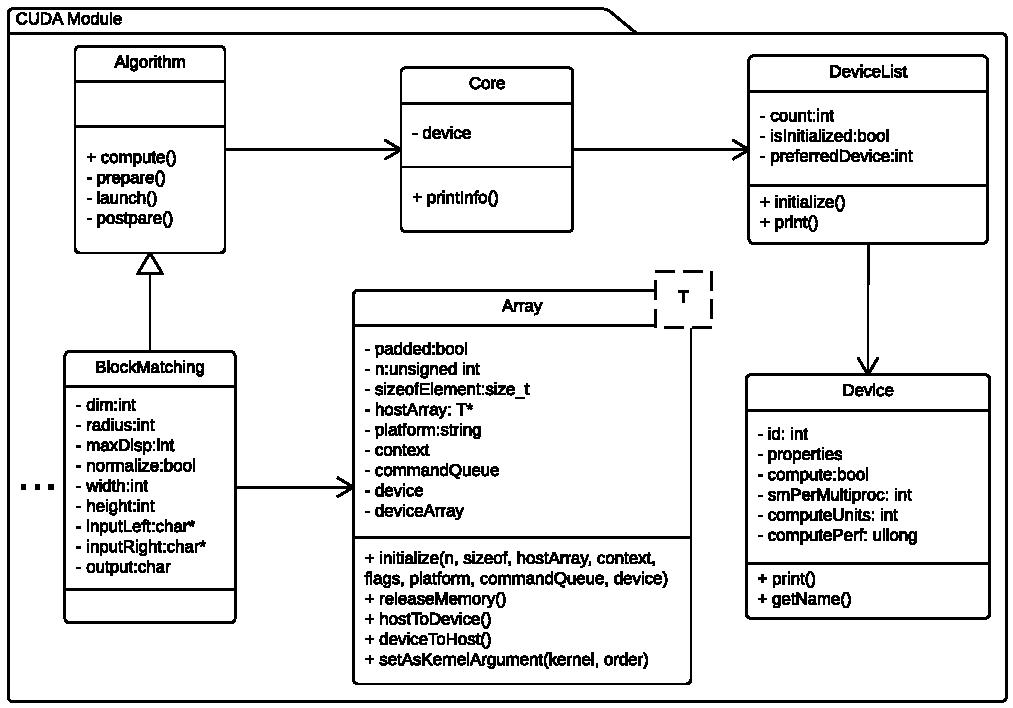
\includegraphics[scale=0.73]{figures/cuda_module.pdf}
	\caption{CUDA module class diagram.} \label{cuda_module}
\end{figure} 

The second GPU computing module gives the user the choice of using CUDA to implement GPU related algorithms using the \textbf{cuda} name space. The most relevant classes explained here are present in the class diagram in \autoref{cuda_module}:

\begin{itemize}
	\item \textbf{Algorithm:} This base class contains the template for the implementation  of CUDA algorithms in GCVL.
	\item \textbf{BlockMatching:} This class serves as an example of the implementation of a CUDA algorithm in GCVL. 
	\item \textbf{Core:} Class in charge of the creation of the CUDA environment, selection of the best GPU, creation device arrays, etc. 
	\item \textbf{Device:} Utility class that aids in the instantiation of compute devices.
	\item \textbf{DevicesList:} Class that holds a list of all the compute devices available in the system. In addition, it tries to guess the best one depending on architecture, compute units and clock speed.
	\item \textbf{Array:} Helper class for CUDA device array creation.
\end{itemize}

\section{Technology}

As mentioned before, GCVL uses the \CC programming language. In order to create a true multi-platform framework, we have also employed the CMake \cite{cmake} build system. The compilers in which the code has been tested are the following:

\begin{itemize}
	\item \textbf{GCC 4.9:} The \textit{GNU Compiler Collection} (GCC) is a compiler system created by the GNU Project supporting various programming languages.
	\item \textbf{Clang 6.1:} This is a compiler front end for C, \CC and other programming languages. It uses LLVM as its back end. 
	\item \textbf{Visual \CC 12.0:} This compiler features tools for developing and debugging C++ code on Microsoft Windows platforms. 
\end{itemize}

For GPGPU programming we have chosen \textbf{OpenCL} and \textbf{CUDA}, because of their inter-operation capabilities with OpenGL. In addition these are the two most used GPGPU frameworks, being OpenCL the leading open source GPGPU framework and CUDA the leading proprietary framework.

In order to keep code versions organized and backed up, \textbf{Git} \cite{gitrev} has been used as a version control system. This  is a distributed revision control system with an emphasis on speed, data integrity, and support for distributed, non-linear work-flows.

Since this is an open source project, we have also used \textbf{GitHub} \cite{github}, a web-based Git repository hosting service. It offers all of the distributed revision control and source code management functionality of Git as well as adding its own features. It provides access control and several collaboration features such as bug tracking, feature requests, task management, and wikis for every project. It is the ideal tool for open source collaboration.

In order to quickly pinpoint issues in the multiple target platforms, we will use the continuous integration tool \textbf{Travis CI}, an open-source hosted and distributed continuous integration service used to build and test projects hosted in GitHub. 

In addition, we have used \textbf{Doxygen} to document the code for maintainability, which is a tool for writing software reference documentation. It is written within the code, and is thus relatively easy to keep up to date and understand. 

%TODO OpenCV, Boost?

\section{Usage}

Once the design concepts behind GCVL and its technology have been explained, the only task left is to know how the modules are used. We will first see how to run the CPU module algorithms, next we will see how the OpenCL tools and algorithms work and last but not least we will see how the CUDA module can be utilized to run the CUDA algorithms.

\subsection{CPU Module}

The CPU module usage is pretty straightforward, one only needs to include the corresponding algorithm class; in our example it will be the BlockMatching algorithm (see \autoref{cpu_bm_example}). In this example, the two paths of the input images and the output image pointer are passed to the BlockMatching class, next the BlockMatching settings are set and the computation is started. The result will be available to the user in the output pointer.

\lstset{language=C++,frame=shadowbox,rulesepcolor=\color[gray]{0.8},lineskip=10pt, 
		keywordstyle=\color{VioletRed}\bfseries,
		emph={Core,BlockMatching}, emphstyle=\color{Emerald}\bfseries, basicstyle=\footnotesize,
		emph={[2]setAggDim,setMaxDisp,setNormalize,compute}, emphstyle={[2]\color{PineGreen}}}
\begin{lstlisting}[float,caption={How to use the BlockMatching class.},captionpos=b,label={cpu_bm_example}]
	#include <gcvl/blockmatching.h>
	int main(int argc, char *argv[]) {
		int dim = 5, maxDisp = 16;
		bool norm = true;
		std::unique_ptr<unsigned char[]> output; 
		gcvl::BlockMatching bm(argv[1], argv[2], output);
		bm.setAggDim(dim);
		bm.setMaxDisp(maxDisp);
		bm.setNormalize(norm);
		bm.compute();
	}
\end{lstlisting}

\subsection{OpenCL Module}

The OpenCL module inner workings are a little more complex, but its usage is still really simple. The first step is to include the corresponding algorithm class and Core class; in our example it will be the BlockMatching algorithm (see \autoref{ocl_bm_example}). In this case, the core, the two paths of the input images and the output image pointer are passed to the BlockMatching class. Next, the BlockMatching settings are set and the computation is started. The result will be available to the user in the output pointer.

\begin{lstlisting}[float,caption={How to use the OpenCL BlockMatching class.},captionpos=b,label={ocl_bm_example}]
	#include <gcvl/opencl/oclcore.h>
	#include <gcvl/opencl/oclblockmatching.h>
	int main(int argc, char *argv[]) {
		int dim = 5, maxDisp = 16;
		bool norm = true;
		std::unique_ptr<unsigned char[]> output;	 
		gcvl::opencl::Core core;
		gcvl::opencl::BlockMatching bm(core, argv[1], argv[2], output);
		bm.setAggDim(dim);
		bm.setMaxDisp(maxDisp);
		bm.setNormalize(norm);
		bm.compute();
	}
\end{lstlisting}

\subsection{CUDA Module}

The CUDA module is used in a similar manner to the OpenCL module, but using a different namespace. The first step is to include the corresponding algorithm class and Core class; in our example it will be the BlockMatching algorithm (see \autoref{cuda_bm_example}). In this case, the core, the two paths of the input images and the output image pointer are passed to the BlockMatching class. Next, the BlockMatching settings are set and the computation is started. The result will be available to the user in the output pointer.

\begin{lstlisting}[float,caption={How to use the CUDA BlockMatching class.},captionpos=b,label={cuda_bm_example}]
	#include <gcvl/cuda/cudacore.h>
	#include <gcvl/cuda/cudablockmatching.h>
	int main(int argc, char *argv[]) {
		int dim = 5, maxDisp = 16;
		bool norm = true;
		std::unique_ptr<unsigned char[]> output;	 
		gcvl::cuda::Core core;
		gcvl::cuda::BlockMatching bm(core, argv[1], argv[2], output);
		bm.setAggDim(dim);
		bm.setMaxDisp(maxDisp);
		bm.setNormalize(norm);
		bm.compute();
	}
\end{lstlisting}
